% ============================================================
%  OPC UA — COURSE SYLLABUS / SELL SHEET
% ============================================================
\documentclass[10pt]{article}
\usepackage[T1]{fontenc}
\usepackage[utf8]{inputenc}
\usepackage{lmodern}
\usepackage{microtype}
\usepackage{palatino}
\usepackage[scaled=0.82]{beramono}
\usepackage[top=0.55in, bottom=0.55in, left=0.65in, right=0.65in]{geometry}
\usepackage[dvipsnames,svgnames,x11names]{xcolor}
\usepackage{tikz}
\usetikzlibrary{positioning,shapes.geometric,arrows.meta,calc,backgrounds,fit}
\usepackage{booktabs}
\usepackage{tabularx}
\usepackage{array}
\usepackage{enumitem}
\usepackage[most]{tcolorbox}
\usepackage{multicol}
\usepackage[colorlinks=true, linkcolor=pblue, urlcolor=pcyan,
  pdftitle={OPC UA — Course Syllabus}]{hyperref}
\usepackage{parskip}

\definecolor{pblue}{HTML}{5B21B6}
\definecolor{pcyan}{HTML}{7C3AED}
\definecolor{pnavy}{HTML}{2E1065}
\definecolor{porange}{HTML}{D97706}
\definecolor{pgreen}{HTML}{15803D}
\definecolor{paccent}{HTML}{F5F3FF}
\definecolor{pgray}{HTML}{6B7280}

\setlength{\parskip}{3pt}
\setlength{\parindent}{0pt}
\pagestyle{empty}

\begin{document}

\begin{tikzpicture}[remember picture, overlay]
  \fill[pnavy] (current page.north west) rectangle ([yshift=-1.05in]current page.north east);
  \node[anchor=west, text=white, font=\fontsize{22}{26}\bfseries\sffamily]
    at ([xshift=0.65in, yshift=-0.38in]current page.north west) {OPC UA};
  \node[anchor=west, text=pcyan!80, font=\fontsize{11}{13}\sffamily]
    at ([xshift=0.65in, yshift=-0.68in]current page.north west) {Study Guide · Industrial Automation Series · SCADA Hub Training Platform};
  \node[anchor=east, draw=pcyan, rounded corners=5pt, fill=pblue!50,
        inner sep=6pt, text=white, font=\small\bfseries\sffamily]
    at ([xshift=-0.65in, yshift=-0.38in]current page.north east)
    {10 Chapters · 600+ Questions · PDF Included};
  \draw[porange, line width=2pt]
    ([xshift=0.65in, yshift=-0.88in]current page.north west) --
    ([xshift=3.5in, yshift=-0.88in]current page.north west);
\end{tikzpicture}

\vspace{0.95in}

\begin{minipage}[t]{0.60\textwidth}

{\color{pnavy}\rule{\linewidth}{1.2pt}}
\smallskip
{\small\sffamily\color{pgray}\MakeUppercase{What This Course Teaches}}
\smallskip

OPC UA is the protocol the entire industry agreed on and almost no one fully understands. It is the integration backbone between PLCs, DCS systems, historians, MES platforms, and cloud analytics — the universal interface layer that replaced decades of proprietary middleware. Engineers who understand OPC UA can connect any compliant system to any other without vendor lock-in. Engineers who do not understand it spend weeks debugging integrations that should take hours.

This course teaches OPC UA from the address space model through security configuration, subscriptions, and session analysis with Wireshark. The emphasis is on what actually matters in production: security modes, session lifecycle, and subscription tuning.

\smallskip
{\color{pblue}\rule{\linewidth}{0.6pt}}
\smallskip
{\small\sffamily\color{pgray}\MakeUppercase{Chapter Sequence}}

\setlist[enumerate]{noitemsep, topsep=2pt, leftmargin=*, label=\textcolor{pblue}{\small\bfseries\arabic*.}}
\begin{enumerate}\small
  \item \textbf{OPC UA Architecture} — Why OPC UA replaced OPC Classic, the unified architecture model, client/server vs.\ pub/sub.
  \item \textbf{Information Model} — Address space, nodes, references, NodeID types, browsing the object hierarchy.
  \item \textbf{Services} — Read, Write, Browse, Subscribe, CreateMonitoredItems, Call — the full service set.
  \item \textbf{Sessions \& Channels} — SecureChannel lifecycle, session establishment, token expiration, reconnect behavior.
  \item \textbf{Security} — Security modes (None/Sign/SignAndEncrypt), certificate exchange, user authentication, PKI infrastructure.
  \item \textbf{Subscriptions} — Publishing interval, sampling interval, deadband filters, queue size, MonitoredItem configuration.
  \item \textbf{Data Types} — Built-in types, structured types, enumerations, arrays, QualityStatusCode interpretation.
  \item \textbf{Discovery} — Local Discovery Server (LDS), Global Discovery Server (GDS), endpoint enumeration.
  \item \textbf{Implementation} — Selecting a stack (open62541 vs.\ commercial), server configuration, common integration patterns.
  \item \textbf{Protocol Lab} — Wireshark OPC UA session analysis, security mode verification, subscription traffic profiling.
\end{enumerate}

\smallskip
{\color{pblue}\rule{\linewidth}{0.6pt}}
\smallskip

{\small\sffamily\color{pgray}\MakeUppercase{The Story}}

\small OPC UA was designed by a committee that included every major automation vendor, intentionally. Every prior integration standard had been owned by a single vendor or consortium. OPC UA is vendor-neutral by construction. The payoff is real: a properly configured OPC UA server exposes every tag, every method, and every alarm to any compliant client — one connection, no custom drivers, no middleware.

The catch is security. OPC UA's security model is sophisticated but optional. Most production deployments use Security Mode None because it was easier during commissioning and nobody changed it. This course teaches engineers to verify, configure, and enforce the correct security mode — and to recognize what a correctly secured OPC UA session looks like in a packet capture.

\end{minipage}
\hfill
\begin{minipage}[t]{0.36\textwidth}

% Address space diagram
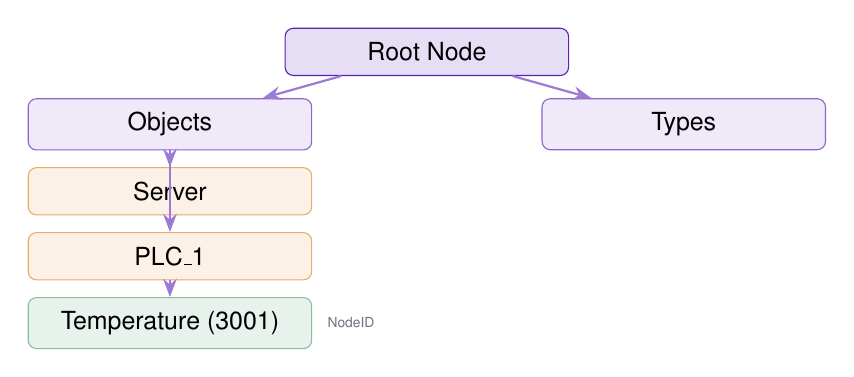
\begin{tikzpicture}[
  node_/.style={rectangle, rounded corners=3pt, text centered,
    font=\small\sffamily, inner sep=5pt, minimum width=3.6cm, minimum height=0.6cm},
  arr/.style={-Stealth, thick, color=pblue!60}
]
\node[node_, fill=pblue!15, draw=pblue] (root) {Root Node};
\node[node_, fill=pblue!10, draw=pblue!70, below left=8pt and -10pt of root] (objs) {Objects};
\node[node_, fill=pblue!10, draw=pblue!70, below right=8pt and -10pt of root] (types) {Types};
\node[node_, fill=porange!10, draw=porange!60, below=6pt of objs] (server) {Server};
\node[node_, fill=porange!10, draw=porange!60, below=6pt of server] (plc) {PLC\_1};
\node[node_, fill=pgreen!10, draw=pgreen!50, below=6pt of plc] (tag) {Temperature (3001)};

\draw[arr] (root) -- (objs);
\draw[arr] (root) -- (types);
\draw[arr] (objs) -- (server);
\draw[arr] (objs) -- (plc);
\draw[arr] (plc) -- (tag);
\node[font=\tiny\sffamily\color{pgray}, right=2pt of tag] {NodeID};
\end{tikzpicture}

\vspace{5pt}

\begin{tcolorbox}[
  enhanced, colback=paccent, colframe=pblue, arc=4pt,
  fonttitle=\small\bfseries\sffamily\color{white},
  title=Certification Relevance,
  boxed title style={colback=pblue},
  attach boxed title to top left={yshift=-2mm, xshift=5mm},
  top=8pt, bottom=6pt, left=6pt, right=6pt
]
\setlist[itemize]{noitemsep, topsep=0pt, leftmargin=*, label=\textcolor{pblue}{$\bullet$}}
\begin{itemize}\small
  \item \textbf{OPC Foundation Certified} — OPC UA Developer \& Integrator certifications directly validate this content.
  \item \textbf{GICSP (GIAC)} — OPC UA security modes and integration patterns appear in ICS security exam prep.
  \item \textbf{ISA CCST} — Industrial networking and integration standards domain.
\end{itemize}
\end{tcolorbox}

\vspace{5pt}

\begin{tcolorbox}[
  enhanced, colback=porange!8, colframe=porange, arc=4pt,
  fonttitle=\small\bfseries\sffamily\color{white},
  title=Next Steps (Certs),
  boxed title style={colback=porange},
  attach boxed title to top left={yshift=-2mm, xshift=5mm},
  top=8pt, bottom=6pt, left=6pt, right=6pt
]
\begin{enumerate}[noitemsep, topsep=0pt, leftmargin=*, label=\small\textcolor{porange}{\arabic*.}]
  \item \small Complete OPC UA + Security guides together.
  \item Review OPC Foundation spec Part 1 (Concepts) and Part 4 (Services).
  \item Apply at \texttt{opcfoundation.org} for Integrator certification exam.
  \item Pair with GICSP for a combined ICS security credential.
\end{enumerate}
\end{tcolorbox}

\vspace{5pt}

\begin{center}
\begin{tikzpicture}
  \foreach \val/\lbl/\col [count=\i] in {
    10/Chapters/pblue,
    600+/Questions/porange,
    3/Levels/pgreen
  }{
    \node[rectangle, rounded corners=3pt, fill=\col!12, draw=\col!40,
          inner sep=5pt, minimum width=1.1cm, font=\sffamily, text=\col] at (\i*1.35, 0)
      {\textbf{\val}\\\tiny\color{pgray}\lbl};
  }
\end{tikzpicture}
\end{center}

\end{minipage}

\begin{tikzpicture}[remember picture, overlay]
  \fill[pnavy!90] (current page.south west) rectangle ([yshift=0.32in]current page.south east);
  \node[anchor=west, text=white!70, font=\footnotesize\sffamily]
    at ([xshift=0.65in, yshift=0.16in]current page.south west)
    {SCADA Hub Training Platform · scada-hub.vercel.app · Free access · No account required for study material};
  \node[anchor=east, text=pcyan, font=\footnotesize\bfseries\sffamily]
    at ([xshift=-0.65in, yshift=0.16in]current page.south east)
    {Course 2 of 8};
\end{tikzpicture}

\end{document}
